\chapter{Návrh a implementace rozšíření}
Rozšíření bude, jak již bylo nastíněno výše, implementováno v jazyce Typescript. K vytvoření rozšíření samotného je potřeba Node.js a Git. Poté je vyžadována instalace programů "Yeoman" a "VS Code Extension Generator", pomocí kterých jsou rozšíření generovány.\\

\section{Error Listener}
Třída, která slouží k detekování zachytávání syntaktických chyb v kódu, čili chyb, které jsou v rozporu z pravidly gramatiky. Každá chyba, kterou rozšíření detekuje, je uložena do struktury ErrorDescription \ref{src:ErrorDescription}. Všechny chyby jsou poté uloženy v poli a pomocí metody getSyntaxErrors() je možné je získat. Rozšíření chyby vypisuje do konzole, jak je ve VS Code zvykem. Sočástí zprávy jsou:
\begin{enumerate}
\item řádek, na kterém se chyba nachází
\item pozice na řádku
\item popis chyby
\end{enumerate}

\begin{lstlisting}[language=Python,label=src:ErrorDescription,caption={rozhraní pro popis chyby}]
export interface ErrorDescription {
	document: string;
	offendingSymbol: any;
	line: number;
	charPositionInLine: number;
	msg : string
	e: RecognitionException | undefined
}
\end{lstlisting}

\section{Modul Toybox}
Komponenta označována, jako modul, představuje v Monkey C jmenný prostor (namespace), pod kterým lze seskupovat třídy, metody, funkce, atd... 
Tento modul tedy obsahuje všechny potřebné třídy, které Monkey C poskytuje, na jednom místě. Z názvů jednotlivých modulů a tříd lze jednoduše odvodit, jaké metody se zde nachází a k jakému účelu slouží.\\ 
Jelikož tento modul, není nikde oficiálně dostupný. Respektive neexistuje žádná oficiální verze, kterou by bylo možné použít, bylo nutné sestavit modul vlastními silami. K jeho vytvoření bylo použito oficiální Connect IQ SDK. V tomto SDK jsou obsaženy informace, ke všem komponentům Toyboxu. Problémem bylo, že zdrojem těchto informací byly soubory ve formátu .html, tedy webové stránky. Bylo tedy nutné veškeré informace extrahovat z html elementů a následně je sestavit do požadované formy.

\section{Zvýraznění kódu}

Zvýraznění, nebo-li obarvení klíčových slov kódu je realizováno pomocí JSON souboru, jenž pomocí regulárních výrazů v textu vyhledává příslušná slova a ty poté obarvuje.
\\
\begin{figure}
	\centering
	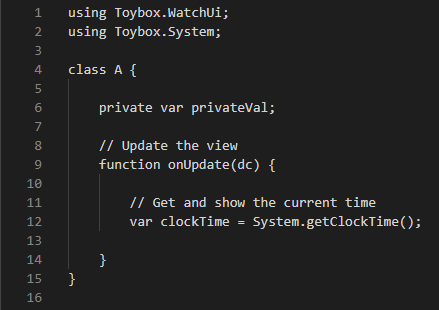
\includegraphics[]{images/uncolored_code}
	\caption{ukázka neobarveného kódu v MonkeyC}
	\label{img:uncolored_code}
\end{figure}

\begin{figure}
	\centering
	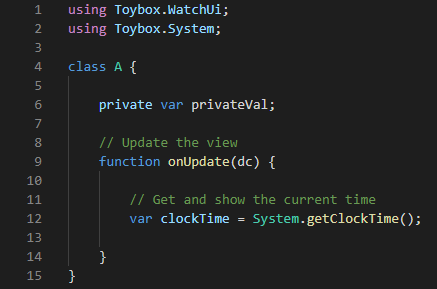
\includegraphics[]{images/colored_code}
	\caption{ukázka obarvení kódu v MonkeyC} 
	\label{img:colored_code}
\end{figure}
	
Hned na první pohled je zřejmé, že obarvení poskytuje uživateli větší přehled a orientaci v kódu, jak je vidět na obrázku \ref{img:colored_code}


\section{Automatické doplňování a našeptávání kódu}
Jako první bylo v rozšíření řešeno našeptávání klíčových slov jazyka, např. NEW, VAR, FUNCTION, atd... k tomuto účelu byl použit "The ANTLR4 Code Completion Core" \cite{mike_lischke}. Jedná se o "stroj" sloužící k dokončování kódu pro analyzátory založené na ANTLR4. Engine c3 je schopen poskytnout kandidáty na doplnění kódu, kteří jsou užiteční pro editory s analyzátory generovanými ANTLR, nezávisle na skutečném jazyku / gramatice použité pro generování. Původní implementace je poskytována jako "node module" a je psána v jazyce Typescript, což bylo vhodné použít vzhledem k tomu, že rozšíření je také psáno v Typescriptu.
\\
Dále bylo řešeno našeptávání lokálních funkcí a proměnných. V Monkey C jsou k tomuto účelu použity 2 prefixy \textbf{self.} a \textbf{me.}. Pokud uživatel v kódu zadá jeden z těchto prefixů, rozšíření spustí funkci \textbf{provideAutocomplete}, která pomocí průchodu syntaktickým stromem všechny dostupné proměnné, funkce, či třídy, podle toho, kde se zrovna uživatel v kódu nachází.
\\
V neposlední řadě bylo potřeba vyřešit, jak zjistit, co se nachází v konkrétní proměnné, a na základě toho poté provést příslušné našeptávání. Toto je řešeno  pomocí komentářů. Tyto Komentáře se objevují jednak v Toyboxu, kde slouží pro orientaci v už tak rozsáhlém modulu a popisu jednotlivých jeho součástí. Součástí popisu jsou informace o datových typech, vstupních parametrech ( pokud se jedná o funkci), návratových typech atd...  
\\
Komentáře má také k dispozici uživatel přímo v kódu. Každá proměnná, která je deklarována, by měla na sebou obsahovat komentář nesoucí informaci o datovém typu této proměnné. Komentář má jednoduchou syntax, viz. \ref{src:comment}, a rozšíření je navíc schopné jeho stukturu automaticky doplnit po zadání "\textbf{/**}". Je zde využito toho, že každá proměnná v Monkey C musí být deklarována předtím, než ji lze použít. A právě na základě tohoto byly v rozšíření komentáře implementovány. Není tedy potřeba složitě hledat a ukládat informace o datovém typu do nějaké struktury, stačí pouze v kanálu komentářů najít příslušný řádek, na kterém je proměnná deklarována a z něj datový typ extrahovat.

\begin{lstlisting}[language=Python,label=src:comment,caption={struktura komentáře datový typ}]
        /**
         * @type Toybox.Lang.Number
         */
\end{lstlisting}

\begin{figure}[h!]
	\centering
	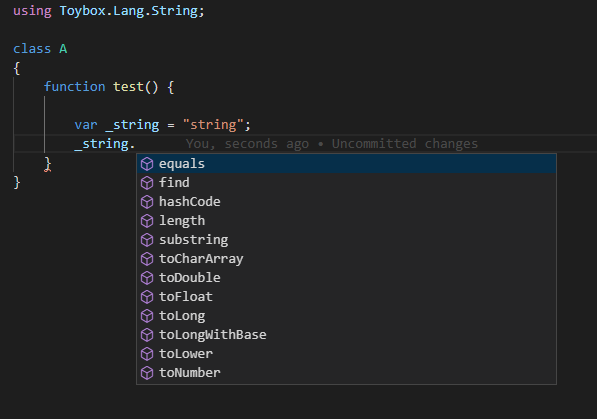
\includegraphics{images/autocomplete_example}
	\caption{ukázka automatického našeptávání kódu na proměnné typy string}
	\label{img:autocomplete_example}
\end{figure}

\begin{figure}
	\centering
	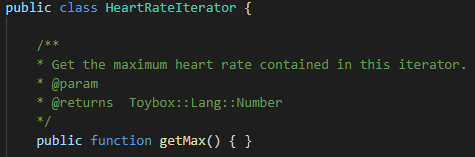
\includegraphics{images/comments}
	\caption{komentář nad funkcí obsahující stručný popis, parametry funkce a návratový typ}
	\label{img:comments}
\end{figure}



\section{Nedostatky rozšíření}
Při implementaci automatického našeptávání byl detekován problém, kvůli kterému není možné provést volání více funkcí po sobě na jednom řádku. Uveďme si příklad, kdy máme proměnnou typu \textbf{String}, v níž je uloženo číslo. Hodnotu v této proměnné budeme chtít převést na typ Integer, čili zavolat metodu \textit{toNumber()}, a poté bezprostředně po volání \textit{toNumber()} zavolat další metodu. Zde nastává problém, kdy rozšíření, jako další vstup neočekává možné volání funkce \ref{img:autocomplete_errormessage}. Jádrem tohoto problému je, že poskytnutá bezkontextová gramatika popisující jazyk není stoprocentně přesná. A právě kvůli těmto "nepřesnostem" je možné při implementaci narazit na podobné komplikace. V průběhu vývoje zatím nebyly registrovány další problémy způsobené gramatikou.

\begin{figure}
	\centering
	
\includegraphics[scale=1]{images/autocomplete_error}
	\caption{nedostatek rozšíření}
	\label{img:autocomplete_error}
\end{figure}

\begin{figure}
	\centering
	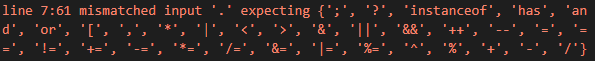
\includegraphics[scale=0.8]{images/autocomplete_errormessage}
	\caption{chybová hláška z error listeneru}
	\label{img:autocomplete_errormessage}
\end{figure}
\endinput